\section{Scatternets}\label{ch:scatternets}
% Let us define the pairs of authors here

  Scatternets have been a very large influence on
  our work, as well as being quite distinct from the previous discussions on
  learned methods. They were first introduced by  
  \citeauthor{bruna_classification_2011} in their work 
  \citep{bruna_classification_2011}, and then were rigorously defined by Mallat
  in \citep{mallat_group_2012}. Several updates and newer models have since
  been released by Mallat's group, which we will review in this chapter.
  
  It is helpful to introduce this chapter with one further note. Unlike the
  CNNs introduced in \autoref{sec:cnns}, which were set up to minimize some
  cost function which had certain constraints to promote certain properties,
  the scattering operator may be thought of as an operator $\Phi$ which has
  some desirable properties for image understanding. These properties may
  ultimately help us minimize some cost function and improve our image
  understanding system, which we explore more in
  \autoref{ch:scat_deep}.


  \section{Translation Invariant Scatternets}
  The translation invariant Scatternets were mostly covered in
  \citep{bruna_invariant_2013}. This section summarises the method of this
  paper.

  \subsection{Defining the Properties}
  The first release of Scatternets aimed at building a translation invariant
  operator, which was also stable to additive noise and deformations. Translation
  is often defined as being uninformative for classification --- an object
  appearing in the centre of the image should be treated the same way as an
  the same object appearing in the corner of an image, i.e.,\ $\Phi x$ is
  invariant to translations $x_c(\bmu{u}) = x(\bmu{u}-\bmu{c})$\footnote{here
  we adopt a slight variation on \Bruna's notation, by using boldface letters to
  represent vectors, as is the custom in Signal Processing} by 
  $\bmu{c}=(c_1,c_2) \in \mathbb{R}^2$ if
  % The first requirement for Scatternets - translation invariance
  \begin{equation}\label{eq:scat_trans_invariance}
    \Phi x_c = \Phi x
  \end{equation}

  Stability to additive noise is another good choice to include in this operator,
  as it is a common feature in measured signals. Stability is defined in terms of
  Lipschitz continuity, which is a strong form of uniform continuity for
  functions, which we briefly introduce here.

  Formally, a Lipschitz continuous function is limited in how fast it can change;
  there exists an upper bound on the gradient the function can take, although it
  doesn't necessarily need to be differentiable everywhere. The modulus operator
  $|x|$ is a good example of a function that has a bounded derivative and so is
  Lipschitz continuous, but isn't differentiable everywhere.

  \begin{figure}
    \begin{center}
      % 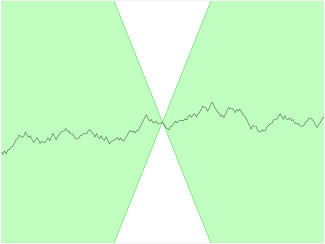
\includegraphics[scale=0.8]{images/Lipschitz_continuity.png}
      \caption[A Lipschitz continuous function]
              {A Lipschitz continuous function is shown. There is a cone for this
              function (shown in white) such that the graph always remains entirely outside
              the cone as it's shifted across. The minimum gradient needed for this to hold
              is called the `best Lipschitz constant'.}
      \label{fig:lipschitz}
    \end{center}
  \end{figure}

  Returning again to stability to additive noise, \Bruna\ state that for a new
  signal $x'(\bmu{u}) = x(\bmu{u}) + \epsilon(\bmu{u})$, there must exist
  a bounded $C>0$ s.t.
  % The second requirement - noise stability
  \begin{equation}\label{eq:scat_noise_stability}
    \|\Phi x' - \Phi x\| \leq C \|x' - x\|
  \end{equation}
  The final requirement is to be stable to small deformations. Enough so that we
  can ignore intra-class variations, but not so invariant that an object can
  morph into another (in the case of MNIST for example, we do not want to be so
  stable to deformations that 7s can map to 1s). Formally, for a new signal
  $x_{\tau}(\bmu{u}) = x(\bmu{u}-\tau(\bmu{u}))$, where $\tau(\bmu{u})$ is a non
  constant displacement field (i.e.,\ not just a translation) that deforms the
  image, we require a $C>0$ s.t.
  % The third requirement - deformation stability
  \protect\begin{equation}\label{eq:scat_deformation_stability}
    \|\Phi x_{\tau} - \Phi x \| \leq C \|x\| \sup_{\bmu{u}} |\nabla\tau(\bmu{u})|
  \protect\end{equation}
  The term on the right $|\nabla\tau(\bmu{u})|$ measures the deformation
  amplitude, so the supremum of it is a limit on the global defomation amplitude.

\subsection{Finding the Right Operator}
  A Fourier modulus satisfies the first two of these requirements, in that it is
  both translation invariant and stable to additive noise, but it is unstable to
  deformations due to the infinite support of the sinusoid basis functions it
  uses. It also loses too much information --- very different signals can all
  have the same Fourier modulus, e.g.\ a chirp, white noise and the Dirac delta
  function all have flat spectra.

  Unlike the Fourier modulus, a wavelet transform
  is stable to deformations due to the grouping together frequencies into dyadic
  packets \citep{mallat_group_2012}, however, the wavelet transform is not invariant to
  shifts. 
  
  We saw in \autoref{ch:freq_analysis} that the modulus of complex, analytic
  wavelets commuted with shifts. The real and imaginary parts are also
  commutative with shifts, but these vary much quicker than the modulus
  (\autoref{fig:pulse_response}).  Interestingly, the modulus operator, in this
  case, does not lose any information \citep{waldspurger_phase_2012} (due to the
  redundancies of the wavelet transform), which is why it may be nice to think
  of it as a \emph{demodulator}.

  \begin{figure}
    \begin{center}
      \newlength\figureheight 
      \newlength\figurewidth 
      \setlength\figureheight{6cm} 
      \setlength\figurewidth{8cm}
      % % This file was created by matlab2tikz.
%
%The latest updates can be retrieved from
%  http://www.mathworks.com/matlabcentral/fileexchange/22022-matlab2tikz-matlab2tikz
%where you can also make suggestions and rate matlab2tikz.
%
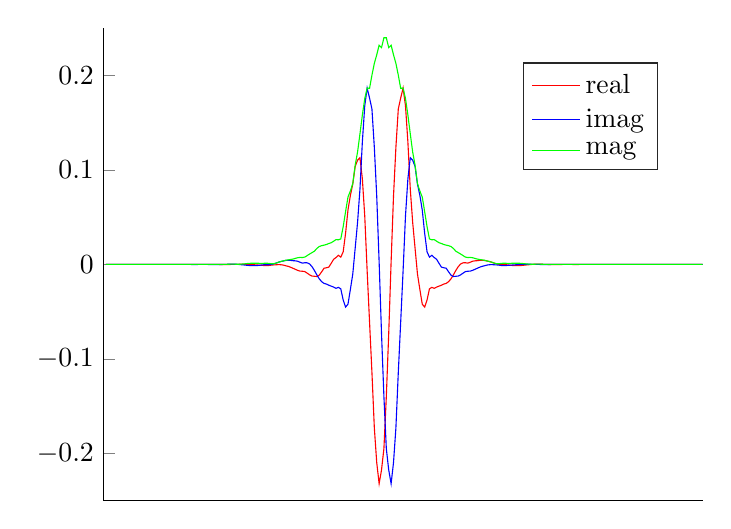
\begin{tikzpicture}

\begin{axis}[%
width=0.951\figurewidth,
height=\figureheight,
at={(0\figurewidth,0\figureheight)},
scale only axis,
xmin=0,
xmax=250,
xtick={\empty},
ymin=-0.25,
ymax=0.25,
axis background/.style={fill=white},
axis x line*=bottom,
axis y line*=left,
legend style={at={(0.7,0.7)},anchor=south west,legend cell align=left,align=left,draw=white!15!black}
]
\addplot [color=red,solid]
  table[row sep=crcr]{%
1	0\\
2	0\\
3	0\\
4	0\\
5	0\\
6	0\\
7	0\\
8	0\\
9	0\\
10	0\\
11	0\\
12	0\\
13	0\\
14	0\\
15	0\\
16	0\\
17	0\\
18	0\\
19	3.40598214094164e-12\\
20	0\\
21	-6.87793140105386e-11\\
22	-9.08261904251105e-11\\
23	4.62741351914918e-10\\
24	1.258882500922e-09\\
25	-3.90768164174049e-09\\
26	-4.94207941791755e-09\\
27	2.25257324923178e-08\\
28	4.47997487754667e-08\\
29	-3.72860948552819e-08\\
30	-7.72685694491778e-08\\
31	1.74091939763211e-07\\
32	3.20701693438365e-07\\
33	6.69906724002732e-08\\
34	-2.57334712035421e-07\\
35	-7.60438752193682e-07\\
36	-6.79175261479185e-07\\
37	3.85670908249705e-07\\
38	1.95760682064202e-06\\
39	2.70916484936271e-06\\
40	3.70985229264904e-06\\
41	5.60263903783335e-06\\
42	7.15200536225569e-06\\
43	9.42804407054984e-06\\
44	9.19816726897712e-06\\
45	4.09312377588624e-06\\
46	-2.18677142696421e-06\\
47	-7.78276608370347e-07\\
48	-2.49334758811333e-06\\
49	-1.24876312688003e-05\\
50	-2.40789294574741e-05\\
51	-5.00285382615212e-05\\
52	-5.19808121979403e-05\\
53	-8.56826227144868e-06\\
54	5.38557733758203e-05\\
55	9.09976831863687e-05\\
56	0.000118256932396166\\
57	0.000164847396440429\\
58	0.000172590561244501\\
59	0.000156541159523113\\
60	7.26324581485654e-05\\
61	-4.32251690266487e-05\\
62	-0.000209156467228341\\
63	-0.000355191843470207\\
64	-0.000528083903626197\\
65	-0.000723523151351148\\
66	-0.000904822353516488\\
67	-0.00117977622340421\\
68	-0.00127386800702199\\
69	-0.00107595626030387\\
70	-0.000731388490979029\\
71	-0.000492950213440953\\
72	-0.000355077529547522\\
73	-0.000176866907141536\\
74	-0.000304238537971187\\
75	-0.000669112865679403\\
76	-0.00137639751374934\\
77	-0.0019999871515232\\
78	-0.00288266647428663\\
79	-0.00399474325488351\\
80	-0.0051470769192401\\
81	-0.00623242432359724\\
82	-0.00706986688887293\\
83	-0.00719378257668194\\
84	-0.00758143497956961\\
85	-0.00925240669242568\\
86	-0.0110384455473666\\
87	-0.0122898662832043\\
88	-0.0125276118821436\\
89	-0.0127859505897159\\
90	-0.0113952391112889\\
91	-0.00784660452604257\\
92	-0.00401960851433002\\
93	-0.00350870901525763\\
94	-0.00282836192466074\\
95	0.00117836761234312\\
96	0.00541190932558586\\
97	0.00731202945632788\\
98	0.00961314726741875\\
99	0.00773250299419411\\
100	0.013341034228591\\
101	0.0329962818862013\\
102	0.0576135809313121\\
103	0.0730546535876305\\
104	0.084986015392322\\
105	0.103631123640744\\
106	0.110327196614011\\
107	0.112909993173503\\
108	0.0905813378752889\\
109	0.0513323912871931\\
110	-0.00674939368285724\\
111	-0.060713087095648\\
112	-0.114305418494503\\
113	-0.17300702433579\\
114	-0.209749288098405\\
115	-0.231992927271329\\
116	-0.217464614066301\\
117	-0.194784442562913\\
118	-0.140070485832163\\
119	-0.0733218645827401\\
120	0.00256331681737184\\
121	0.0722909879534431\\
122	0.123938750062336\\
123	0.164537100743611\\
124	0.1761522691017\\
125	0.186614921947609\\
126	0.16786851431561\\
127	0.129648576703118\\
128	0.0797149042875755\\
129	0.0445213447780424\\
130	0.0170433369608732\\
131	-0.0101767458153209\\
132	-0.0264788340863422\\
133	-0.0420467635360721\\
134	-0.0451140888775753\\
135	-0.0376649209952693\\
136	-0.0258341146252317\\
137	-0.0242550663754605\\
138	-0.0252504924158299\\
139	-0.0239210066309461\\
140	-0.0229612977291479\\
141	-0.0220048369351539\\
142	-0.0207817770698637\\
143	-0.0200383376462408\\
144	-0.0182129976759503\\
145	-0.0151705843558306\\
146	-0.0110133286799118\\
147	-0.00640572486704498\\
148	-0.00241914987168933\\
149	0.000501553892557113\\
150	0.00171502644229679\\
151	0.00182682703744143\\
152	0.00135819388712596\\
153	0.0023202015883891\\
154	0.00338143714657009\\
155	0.0038167928839548\\
156	0.00398922920965832\\
157	0.00435012390937784\\
158	0.00438744590069432\\
159	0.00420434222714658\\
160	0.00365909375507545\\
161	0.0031096699498426\\
162	0.00234243116660081\\
163	0.00139821952573963\\
164	0.000556075684303888\\
165	-5.51706115206466e-05\\
166	-0.000331691562229006\\
167	-0.000361308885120112\\
168	-0.00030880647995183\\
169	-0.000606048853947934\\
170	-0.000942240424391602\\
171	-0.00116480277977496\\
172	-0.00125325781851377\\
173	-0.00129181029001784\\
174	-0.00115716277061801\\
175	-0.000949777311562008\\
176	-0.000655071283282308\\
177	-0.000401238951280002\\
178	-0.000168066677392165\\
179	7.51939646498624e-05\\
180	0.000224400979048634\\
181	0.000325006343811925\\
182	0.00029951693903595\\
183	0.000193407642771761\\
184	5.23403692689068e-05\\
185	-7.08866952670796e-07\\
186	-1.49391620378925e-05\\
187	-3.63681852437294e-05\\
188	-3.66387543450729e-05\\
189	-4.31719371365099e-05\\
190	-3.68830397411496e-05\\
191	-1.45273881114298e-05\\
192	7.69634724727019e-06\\
193	1.40718734743013e-05\\
194	9.47996727945057e-06\\
195	1.08877455419357e-06\\
196	-8.37952554555356e-06\\
197	-9.54752048564336e-06\\
198	-6.25889587127397e-06\\
199	-2.89688757013566e-06\\
200	7.1722847502998e-07\\
201	1.69289428040498e-06\\
202	1.08252608403094e-06\\
203	5.10006804932853e-07\\
204	-3.13462849361191e-07\\
205	-3.54749535554903e-07\\
206	-1.07355897601877e-07\\
207	-3.86544340676565e-08\\
208	4.33594828396285e-08\\
209	5.64209933272261e-08\\
210	2.65249108795441e-08\\
211	1.4160405157173e-08\\
212	-9.40796883785182e-10\\
213	-2.76659516509318e-09\\
214	1.45966616149977e-09\\
215	3.51734339084897e-10\\
216	-1.27226347003132e-10\\
217	-8.49537384694854e-11\\
218	0\\
219	4.77098801261746e-12\\
220	0\\
221	0\\
222	0\\
223	0\\
224	0\\
225	0\\
226	0\\
227	0\\
228	0\\
229	0\\
230	0\\
231	0\\
232	0\\
233	0\\
234	0\\
235	0\\
236	0\\
237	0\\
238	0\\
239	0\\
240	0\\
241	0\\
242	0\\
243	0\\
244	0\\
245	0\\
246	0\\
247	0\\
248	0\\
249	0\\
250	0\\
};
\addlegendentry{real};

\addplot [color=blue,solid]
  table[row sep=crcr]{%
1	0\\
2	0\\
3	0\\
4	0\\
5	0\\
6	0\\
7	0\\
8	0\\
9	0\\
10	0\\
11	0\\
12	0\\
13	0\\
14	0\\
15	0\\
16	4.77098801261746e-12\\
17	0\\
18	-8.49537384694854e-11\\
19	-1.27226347003132e-10\\
20	3.51734339084897e-10\\
21	1.45966616149977e-09\\
22	-2.76659516509318e-09\\
23	-9.40796883785182e-10\\
24	1.4160405157173e-08\\
25	2.65249108795441e-08\\
26	5.64209933272261e-08\\
27	4.33594828396285e-08\\
28	-3.86544340676565e-08\\
29	-1.07355897601877e-07\\
30	-3.54749535554903e-07\\
31	-3.13462849361191e-07\\
32	5.10006804932853e-07\\
33	1.08252608403094e-06\\
34	1.69289428040498e-06\\
35	7.1722847502998e-07\\
36	-2.89688757013566e-06\\
37	-6.25889587127397e-06\\
38	-9.54752048564336e-06\\
39	-8.37952554555356e-06\\
40	1.08877455419357e-06\\
41	9.47996727945057e-06\\
42	1.40718734743013e-05\\
43	7.69634724727019e-06\\
44	-1.45273881114298e-05\\
45	-3.68830397411496e-05\\
46	-4.31719371365099e-05\\
47	-3.66387543450729e-05\\
48	-3.63681852437294e-05\\
49	-1.49391620378925e-05\\
50	-7.08866952670774e-07\\
51	5.23403692689068e-05\\
52	0.000193407642771761\\
53	0.00029951693903595\\
54	0.000325006343811925\\
55	0.000224400979048634\\
56	7.51939646498624e-05\\
57	-0.000168066677392165\\
58	-0.000401238951280002\\
59	-0.000655071283282308\\
60	-0.000949777311562008\\
61	-0.00115716277061801\\
62	-0.00129181029001784\\
63	-0.00125325781851377\\
64	-0.00116480277977496\\
65	-0.000942240424391602\\
66	-0.000606048853947934\\
67	-0.00030880647995183\\
68	-0.000361308885120112\\
69	-0.000331691562229006\\
70	-5.51706115206467e-05\\
71	0.000556075684303888\\
72	0.00139821952573963\\
73	0.00234243116660081\\
74	0.0031096699498426\\
75	0.00365909375507545\\
76	0.00420434222714658\\
77	0.00438744590069432\\
78	0.00435012390937784\\
79	0.00398922920965832\\
80	0.0038167928839548\\
81	0.00338143714657009\\
82	0.0023202015883891\\
83	0.00135819388712596\\
84	0.00182682703744143\\
85	0.0017150264422968\\
86	0.000501553892557114\\
87	-0.00241914987168932\\
88	-0.00640572486704498\\
89	-0.0110133286799118\\
90	-0.0151705843558306\\
91	-0.0182129976759503\\
92	-0.0200383376462408\\
93	-0.0207817770698637\\
94	-0.0220048369351539\\
95	-0.0229612977291479\\
96	-0.0239210066309461\\
97	-0.0252504924158299\\
98	-0.0242550663754605\\
99	-0.0258341146252317\\
100	-0.0376649209952693\\
101	-0.0451140888775753\\
102	-0.0420467635360721\\
103	-0.0264788340863422\\
104	-0.0101767458153209\\
105	0.0170433369608732\\
106	0.0445213447780424\\
107	0.0797149042875755\\
108	0.129648576703118\\
109	0.16786851431561\\
110	0.186614921947609\\
111	0.1761522691017\\
112	0.164537100743611\\
113	0.123938750062336\\
114	0.0722909879534431\\
115	0.00256331681737185\\
116	-0.0733218645827401\\
117	-0.140070485832163\\
118	-0.194784442562913\\
119	-0.217464614066301\\
120	-0.231992927271329\\
121	-0.209749288098405\\
122	-0.17300702433579\\
123	-0.114305418494503\\
124	-0.0607130870956479\\
125	-0.00674939368285723\\
126	0.0513323912871931\\
127	0.0905813378752889\\
128	0.112909993173503\\
129	0.110327196614011\\
130	0.103631123640744\\
131	0.0849860153923221\\
132	0.0730546535876306\\
133	0.0576135809313121\\
134	0.0329962818862013\\
135	0.013341034228591\\
136	0.00773250299419411\\
137	0.00961314726741875\\
138	0.00731202945632788\\
139	0.00541190932558586\\
140	0.00117836761234312\\
141	-0.00282836192466074\\
142	-0.00350870901525763\\
143	-0.00401960851433002\\
144	-0.00784660452604257\\
145	-0.0113952391112889\\
146	-0.0127859505897159\\
147	-0.0125276118821436\\
148	-0.0122898662832043\\
149	-0.0110384455473666\\
150	-0.00925240669242567\\
151	-0.00758143497956961\\
152	-0.00719378257668194\\
153	-0.00706986688887293\\
154	-0.00623242432359725\\
155	-0.00514707691924009\\
156	-0.00399474325488351\\
157	-0.00288266647428663\\
158	-0.0019999871515232\\
159	-0.00137639751374934\\
160	-0.000669112865679403\\
161	-0.000304238537971186\\
162	-0.000176866907141536\\
163	-0.000355077529547522\\
164	-0.000492950213440953\\
165	-0.000731388490979029\\
166	-0.00107595626030387\\
167	-0.00127386800702199\\
168	-0.00117977622340421\\
169	-0.000904822353516488\\
170	-0.000723523151351148\\
171	-0.000528083903626196\\
172	-0.000355191843470207\\
173	-0.000209156467228341\\
174	-4.32251690266487e-05\\
175	7.26324581485654e-05\\
176	0.000156541159523113\\
177	0.000172590561244501\\
178	0.000164847396440429\\
179	0.000118256932396166\\
180	9.09976831863687e-05\\
181	5.38557733758203e-05\\
182	-8.56826227144868e-06\\
183	-5.19808121979403e-05\\
184	-5.00285382615212e-05\\
185	-2.40789294574741e-05\\
186	-1.24876312688003e-05\\
187	-2.49334758811333e-06\\
188	-7.78276608370347e-07\\
189	-2.18677142696421e-06\\
190	4.09312377588625e-06\\
191	9.19816726897713e-06\\
192	9.42804407054984e-06\\
193	7.15200536225569e-06\\
194	5.60263903783335e-06\\
195	3.70985229264904e-06\\
196	2.70916484936271e-06\\
197	1.95760682064202e-06\\
198	3.85670908249705e-07\\
199	-6.79175261479185e-07\\
200	-7.60438752193682e-07\\
201	-2.57334712035421e-07\\
202	6.69906724002732e-08\\
203	3.20701693438365e-07\\
204	1.74091939763211e-07\\
205	-7.72685694491778e-08\\
206	-3.72860948552819e-08\\
207	4.47997487754667e-08\\
208	2.25257324923178e-08\\
209	-4.94207941791755e-09\\
210	-3.90768164174049e-09\\
211	1.258882500922e-09\\
212	4.62741351914918e-10\\
213	-9.08261904251105e-11\\
214	-6.87793140105386e-11\\
215	0\\
216	3.40598214094164e-12\\
217	0\\
218	0\\
219	0\\
220	0\\
221	0\\
222	0\\
223	0\\
224	0\\
225	0\\
226	0\\
227	0\\
228	0\\
229	0\\
230	0\\
231	0\\
232	0\\
233	0\\
234	0\\
235	0\\
236	0\\
237	0\\
238	0\\
239	0\\
240	0\\
241	0\\
242	0\\
243	0\\
244	0\\
245	0\\
246	0\\
247	0\\
248	0\\
249	0\\
250	0\\
};
\addlegendentry{imag};

\addplot [color=green,solid]
  table[row sep=crcr]{%
1	0\\
2	0\\
3	0\\
4	0\\
5	0\\
6	0\\
7	0\\
8	0\\
9	0\\
10	0\\
11	0\\
12	0\\
13	0\\
14	0\\
15	0\\
16	4.77098801261746e-12\\
17	0\\
18	8.49537384694854e-11\\
19	1.27271929686423e-10\\
20	3.51734339084897e-10\\
21	1.46128570001326e-09\\
22	2.76808565698103e-09\\
23	1.04844090692416e-09\\
24	1.42162533519356e-08\\
25	2.6811207973177e-08\\
26	5.66370253191664e-08\\
27	4.88615736180845e-08\\
28	5.91707931621314e-08\\
29	1.13646564485961e-07\\
30	3.6306702521868e-07\\
31	3.5856235360137e-07\\
32	6.02458726596314e-07\\
33	1.08459691719828e-06\\
34	1.7123411455216e-06\\
35	1.04531515880701e-06\\
36	2.97543889700524e-06\\
37	6.27076706447628e-06\\
38	9.74614651480286e-06\\
39	8.80658972302032e-06\\
40	3.86632048117235e-06\\
41	1.1011782045051e-05\\
42	1.57850816842511e-05\\
43	1.21705289920691e-05\\
44	1.71945132658123e-05\\
45	3.71094635206701e-05\\
46	4.32272845017189e-05\\
47	3.66470194482135e-05\\
48	3.64535551094453e-05\\
49	1.9470991168914e-05\\
50	2.40893614729532e-05\\
51	7.24042049593117e-05\\
52	0.00020027111903439\\
53	0.000299639469843039\\
54	0.000329438261050387\\
55	0.000242149494617008\\
56	0.000140138625580231\\
57	0.000235416805183551\\
58	0.000436783925820271\\
59	0.000673515791059104\\
60	0.000952550479258007\\
61	0.00115796981521183\\
62	0.00130863297114945\\
63	0.00130261905610722\\
64	0.0012789206875489\\
65	0.00118798264629529\\
66	0.00108903567654817\\
67	0.00121952178306504\\
68	0.00132411623726202\\
69	0.00112592236257258\\
70	0.00073346637353879\\
71	0.000743115118676452\\
72	0.00144260108628446\\
73	0.00234909890662455\\
74	0.00312451728830885\\
75	0.00371976869381013\\
76	0.0044239081905961\\
77	0.00482178702741808\\
78	0.00521855765790864\\
79	0.00564552241689185\\
80	0.00640783182766075\\
81	0.00709064384421969\\
82	0.007440857023028\\
83	0.0073208741551538\\
84	0.0077984263396001\\
85	0.00941001303398782\\
86	0.0110498342254224\\
87	0.0125256975598461\\
88	0.01407033654686\\
89	0.0168752464009988\\
90	0.0189736159996144\\
91	0.0198313511121225\\
92	0.0204375201096715\\
93	0.0210758937446378\\
94	0.0221858621585816\\
95	0.0229915146007476\\
96	0.024525564637458\\
97	0.026287889645464\\
98	0.0260906275367817\\
99	0.0269665177771404\\
100	0.0399578461365013\\
101	0.0558930732163425\\
102	0.0713249958400785\\
103	0.0777052833813811\\
104	0.0855931595844764\\
105	0.105023259908484\\
106	0.118971595154272\\
107	0.138214082220365\\
108	0.158157302115399\\
109	0.17554159761661\\
110	0.186736936380028\\
111	0.186321498637064\\
112	0.200345167693949\\
113	0.212819745880261\\
114	0.221857501106166\\
115	0.232007088031867\\
116	0.229492819488748\\
117	0.239918152847597\\
118	0.239918152847597\\
119	0.229492819488748\\
120	0.232007088031867\\
121	0.221857501106166\\
122	0.212819745880261\\
123	0.200345167693949\\
124	0.186321498637064\\
125	0.186736936380028\\
126	0.17554159761661\\
127	0.158157302115399\\
128	0.138214082220365\\
129	0.118971595154272\\
130	0.105023259908484\\
131	0.0855931595844765\\
132	0.0777052833813811\\
133	0.0713249958400785\\
134	0.0558930732163425\\
135	0.0399578461365013\\
136	0.0269665177771404\\
137	0.0260906275367817\\
138	0.026287889645464\\
139	0.024525564637458\\
140	0.0229915146007476\\
141	0.0221858621585816\\
142	0.0210758937446378\\
143	0.0204375201096715\\
144	0.0198313511121225\\
145	0.0189736159996144\\
146	0.0168752464009988\\
147	0.01407033654686\\
148	0.0125256975598461\\
149	0.0110498342254224\\
150	0.00941001303398781\\
151	0.0077984263396001\\
152	0.00732087415515381\\
153	0.007440857023028\\
154	0.0070906438442197\\
155	0.00640783182766075\\
156	0.00564552241689185\\
157	0.00521855765790864\\
158	0.00482178702741808\\
159	0.0044239081905961\\
160	0.00371976869381013\\
161	0.00312451728830885\\
162	0.00234909890662455\\
163	0.00144260108628446\\
164	0.000743115118676453\\
165	0.00073346637353879\\
166	0.00112592236257258\\
167	0.00132411623726202\\
168	0.00121952178306504\\
169	0.00108903567654817\\
170	0.00118798264629529\\
171	0.0012789206875489\\
172	0.00130261905610722\\
173	0.00130863297114945\\
174	0.00115796981521183\\
175	0.000952550479258007\\
176	0.000673515791059104\\
177	0.000436783925820271\\
178	0.000235416805183551\\
179	0.000140138625580231\\
180	0.000242149494617008\\
181	0.000329438261050387\\
182	0.000299639469843039\\
183	0.00020027111903439\\
184	7.24042049593117e-05\\
185	2.40893614729532e-05\\
186	1.9470991168914e-05\\
187	3.64535551094453e-05\\
188	3.66470194482135e-05\\
189	4.32272845017189e-05\\
190	3.71094635206701e-05\\
191	1.71945132658123e-05\\
192	1.21705289920691e-05\\
193	1.57850816842511e-05\\
194	1.1011782045051e-05\\
195	3.86632048117234e-06\\
196	8.80658972302032e-06\\
197	9.74614651480286e-06\\
198	6.27076706447628e-06\\
199	2.97543889700524e-06\\
200	1.04531515880701e-06\\
201	1.7123411455216e-06\\
202	1.08459691719828e-06\\
203	6.02458726596314e-07\\
204	3.5856235360137e-07\\
205	3.6306702521868e-07\\
206	1.13646564485961e-07\\
207	5.91707931621314e-08\\
208	4.88615736180845e-08\\
209	5.66370253191664e-08\\
210	2.6811207973177e-08\\
211	1.42162533519356e-08\\
212	1.04844090692416e-09\\
213	2.76808565698103e-09\\
214	1.46128570001326e-09\\
215	3.51734339084897e-10\\
216	1.27271929686423e-10\\
217	8.49537384694854e-11\\
218	0\\
219	4.77098801261746e-12\\
220	0\\
221	0\\
222	0\\
223	0\\
224	0\\
225	0\\
226	0\\
227	0\\
228	0\\
229	0\\
230	0\\
231	0\\
232	0\\
233	0\\
234	0\\
235	0\\
236	0\\
237	0\\
238	0\\
239	0\\
240	0\\
241	0\\
242	0\\
243	0\\
244	0\\
245	0\\
246	0\\
247	0\\
248	0\\
249	0\\
250	0\\
};
\addlegendentry{mag};

\end{axis}
\end{tikzpicture}% 
      \caption{Real, Imaginary and Modulus of complex wavelet convolved with
               an impulse.}
      \label{fig:pulse_response}
    \end{center}
  \end{figure}
  

  % A tikz diagram to draw what the operator looks like so far
  %\input{tikz/invariant}

  The modulus can be made fully invariant by integrating, i.e.,:
  $$\int F x(\bmu{u})d\bmu{u}= \int | x \ast \psi_{\lambda}(\bmu{u})| d\bmu{u}$$
  is translation invariant. 
  Total invariance to shifts means integrating over the entire function, which
  may not be ideal as it loses a significant amount of information in doing this. Instead
  \citeauthor{bruna_invariant_2013} define scales $2^J$, over which their operator
  is invariant to shifts. Now instead of integrating, the output $\|x \ast \psi_{\lambda}\|$ is
  convolved with an averaging window, or conveniently, the scaling function for
  the chosen wavelet:
  $$\phi_{2^J}(\bmu{u}) = 2^{-2J}\phi(2^{-J}\bmu{u})$$

  Even still, this averaging means that a lot of information is lost from the
  first layer outputs ($\|x \ast \psi_{\lambda}\|$).
  \citeauthor{bruna_invariant_2013} combat this by also convolving the output
  with wavelets that cover the rest of the frequency space, giving  
  $$U[p]x = U[\lambda_2]U[\lambda_1]x = \| | x \ast \psi_{\lambda_1}| 
    \ast \psi_{\lambda_2} \|$$
  The choice of wavelet functions $\lambda_{1}$ and $\lambda_{2}$ is combined
  into a path variable, $p = (\lambda_1, \lambda_2, \ldots \lambda{m})$.

  Local invariants can be again computed by convolving this with another scaling
  function $\phi$. The result is now a multiscale scattering transform, with
  coefficients:
  $$ S[p]x = U[p]x \ast \phi_{2^J}(\bmu{u}) $$
  A graphical representation of this is shown in
  \autoref{fig:scatternet_mallat}.

  \begin{figure}
    \centering
      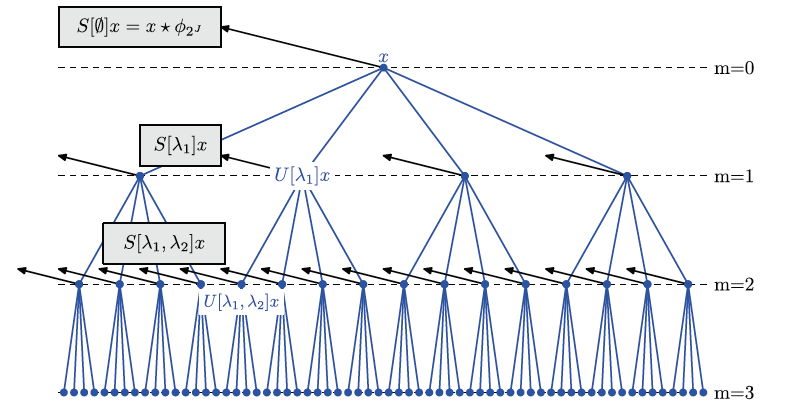
\includegraphics[width=\textwidth]{images/scatternet_diagram.png}
      \caption[Translation Invariant Scatternet Layout]
              {The translation invariant Scattering Transform. Scattering outputs
               are the leftward pointing arrows $S[p]x$, and the intermediate 
               coefficients $U[p]x$ are the centre nodes of the tree. Taken
               from \citep{bruna_invariant_2013}.}
      \label{fig:scatternet_mallat}
  \end{figure}

  % \begin{eqnarray*}
  % \bm{lambda} &=& (j, \theta)
  % % Scattering transform equation
  % \begin{eqnarray*}
  % \Phi x & = & \{S[\bmu{p}]x(\bmu{u}) | \bmu{p} = (\bmu{\lambda_{1}},
  % \bmu{\lambda_{2}}, \ldots \bmu{\lambda_{m}})

\section{Rotation and Translation Invariant Scatternets}
  Mallat's group refined their Scatternet architecture by expanding their list
  of invariants to also include rotation. They also experimented with adding
  scale invariance in \citep{sifre_rotation_2013}, but it was limited to only
  averaging over scale once, and they were no longer using
  it in \citep{oyallon_deep_2015}, so for brevity we omit it. 
  
  This work was done by two authors, each tackling different
  challenges. The first is texture analysis with Sifre in
  \citep{sifre_combined_2012, sifre_rotation_2013, sifre_rigid-motion_2014,
  sifre_rigid-motion_2014-1}, and the second is image classification with
  Oyallon in \citep{oyallon_generic_2013, oyallon_deep_2015}. In this section,
  we outline the properties and structure of this extended Scatternet.

\subsection{An Important note on Joint vs. Separable Invariants}
  When building multiple invariants, some thought must be given as to how to
  combine them --- separably or jointly? Let us call the group of operations we
  want to be invariant to $G$, with $g \in G$ a single realization from this
  group --- in this case, $G$ is the group of affine transformations. We want
  our operator $\Phi$ to be invariant to all  $g \in G$, i.e.,\ $\Phi(gx)
  = \Phi(x)$. Building separable invariants would mean representing the group
  as $G=G_2G_1$ (an assumption of the group, not of our model), and building
  $\Phi = \Phi_2 \Phi_1$, where $\Phi_1$ is invariant to members of $G_1$ and
  covariant to members of $G_2$, and $\Phi_2$ is invariant to members of $G_2$.
  I.e.,\
  \begin{equation}
    \Phi_2(\Phi_1(g_1g_2x)) = \Phi_2(g_2\Phi_1(x)) = \Phi_2(\Phi_1(x))
  \end{equation}
  An example of this would be in the group $G$ of 2D translations, building
  horizontal invariance first, then building vertical invariance second.
  \Bruna\ warn about this approach, however, as it cannot capture the action
  of $G_2$ relative to $G_1$. In the case of veritcal and horizontal
  translations, for example, it would not be able to distinguish if the
  patterns had moved apart as well as being shifted, whereas a joint
  horizontal and vertical translation invariant would be able to distinguish
  these two cases.

  % \begin{figure}[t!]
    % \centering
  % %    \captionsetup[subfigure]{width=0.3\textwdith}
      % \subfloat[]{\includegraphics[width=0.3\textwidth]{scripts/separable_invariance_1.png}
                  % \label{fig:joint_pattern1}}
  % %    \quad   
      % \subfloat[]{\includegraphics[width=0.3\textwidth]{scripts/separable_invariance_2.png}
                  % \label{fig:joint_pattern2}}
  % %    \quad
      % \subfloat[]{\includegraphics[width=0.3\textwidth]{scripts/separable_invariance_3.png}
                  % \label{fig:joint_pattern3}}
      % \caption[Patterns illustrating the difference between joint and separable invariants]
              % {Patterns illustrating the difference between joint and separable
              % invariants. \subref{fig:joint_pattern1} the reference pattern.
              % \subref{fig:joint_pattern2} pattern shifted horizontally and
              % vertically.  \subref{fig:joint_pattern3} pattern shifted apart.
              % A joint invariant would be able to distinguish
              % between~\subref{fig:joint_pattern2}
              % and~\subref{fig:joint_pattern3}, but a separable invariant would
              % not.}
      % \label{fig:joint_pattern}
  % \end{figure}

  In this vein, \Bruna\ suggest that in the case of rotation and translation
  invariance, a joint invariant should be used, building on the work in
  \citep{citti_cortical_2006, boscain_anthropomorphic_2010,
  sgallari_scale_2007}. 

  % \begin{figure}
    % \centering
      % \includegraphics[width=7cm]{images/scatternet_roto_scale_block.png}
      % \caption{Roto-Translation and Scale Invariant Scatternet block diagram. The
               % log operation between roto-translation and scale invariances is used to
               % linearize the power law of the Scatternet coefficient energies across 
               % scales. Taken from \citep{sifre_rotation_2013}.}
      % \label{fig:roto_scat_block}
  % \end{figure}

\subsection{Defining the Properties}
  A translation $g = (v, \theta)$ of the roto-translation group $G_{rt}$ acting on
  $\bmu{u} \in \mathbb{R}^2$ combines translation by $v$ and rotation by
  $R_{\theta}$ as:
  \begin{equation}
    g\bmu{u} = v + R_{\theta}\bmu{u}
  \end{equation}
  The product of two successive roto-translations $h=(v',
  \theta ')$ and $g = (v, \theta) $is:
  \begin{equation}
    gh = (v + R_{\theta}v', \theta + \theta')
  \end{equation}
  In much the similar approach to the simple translation invariant Scatternet defined
  above, \Bruna\ calculate successive layers of signal coefficients $U[p]x$ that
  are covariant to the actions of all $g \in G_{rt}$ --- i.e.,\ 
  \begin{equation}
    U[p](gx) = gU[p]x
  \end{equation}
  Creating invariants of order $m = \mathrm{length}(p)
  = \mathrm{length}([\lambda_1, \lambda_2, \ldots, \lambda_m])$ is then done by
  averaging $hU[p]x$ for all h in $G_{rt}$
  \begin{equation}
    S[p]x(g) = \sum_{h \in G_{rt}} hU[p]x \Phi_J(h^{-1}g)
  \end{equation}
  This convolution averages $hU[p]x$ over all rotation angles in a spatial
  neighbourhood of $\bmu{u}$ of size proportional to $2^J$.

\subsection{The Operator}
\subsubsection{Roto-Translation Invariance}
  Although we want to have a joint invariant for rotations and translations,
  this can be done with a cascade of wavelet transforms --- so long as the
  final averaging operation is done over both rotation and translation. \Sifre\
  do just this, building a 3 layer scattering transform, the first layer of
  which is exactly identical to the previous translation scattering transform,
  i.e.,\
  \begin{equation}
    \tilde{W}_1 x = \left( x \ast \phi_J, \{|x \ast \psi_{\theta, j}|\} \right)
      = (S_0x, U_1x)
  \end{equation}
  The second and third layers are, however, new. The invariant part of $U_1$ is
  computed with an averaging over spatial and angle variables. \emph{This
  averaging is implemented at fixed scales j} (see our note earlier about
  choosing separable scale invariance). For an action $g = (v, \theta)$, the
  averaging kernel is defined as:
  \begin{equation}
    \Phi_J(g) =  \bar{\phi}(\theta) \ast \phi_J(u)
  \end{equation}
  Where $\phi_J(u)$ is a kernel that averages each $U_1x$ over scale $2^J$,
  and $ \bar{\phi}(\theta= (2\pi)^{-1})$ averages the result of that average over all angles.

  To clarify, we look at an example architecture with $J=2$ scales and $L=4$
  orientations. The output of the first layer $U_1x$ would be a set of
  coefficients:
  \begin{equation}
    U_1x = \left\{ |x \ast \psi_{j, \theta} | \, \middle| \, j=\{0,1\}, \,
    \theta=k\pi/4, \, k= \{0,1,2,3\} ,\right\}
  \end{equation}
  i.e.,\ there would be 4 high frequency coefficients, which were created with
  wavelets centred at $|\bm{\omega}| = 3\pi/4$, and 4 medium frequency components
  created with wavelets centred at $|\bm{\omega}| = 3\pi/8$. Each of these 8 will
  be averaged across the entire image, then each pair of 4 will be averaged
  across all 4 rotations, leaving 2 invariants.

  To recover the information lost from averaging, \Sifre\ also convolve $U_1x$
  with corresponding rotation and scale wavelets to pass on the high frequency
  information. These roto-translation wavelets, while joint, can also be computed
  with the cascade of separable wavelets. It may be helpful to consider the
  spatial variable $\bmu{u}$ as single dimensional, and consider the rotation
  variable $\theta$ as a second dimension. The above equation calculated the low-low
  frequency component of these two variables, the remaining components are the
  low-high, high-low, and high-high. 

  We define the low frequency spatial scaling functions $\phi_J(u)$\footnote{we
  temporarily drop the boldface from the spatial parameter u to make it clearer
  it can be considered as single dimensional}, the spatial wavelets
  $\psi_{\theta, j}(u)$, the rotation scaling function $\bar{\phi}(\theta)$
  (which is just the constant $(2\pi)^{-1}$, but we write out in generic form
  nonetheless), and the rotation wavelet $\bar{\psi}_k(\theta)$, which is
  a $2\pi$ periodic wavelet.

  Then, the remaining low-high, high-low, and high-high information is:
  \begin{eqnarray}
    \Psi_{0, J, k_2}(u, \theta) & = & \phi_J(u) \ast \bar{\psi}_{k_2}(\theta) \\
    \Psi_{\theta_2, j_2, } (u, \theta) & = & \psi_{\theta_2, j_2}(u) \ast
      \bar{\phi}(\theta) \\
    \Psi_{\theta_2, j_2, k_2}(u, \theta) & = & \psi_{\theta_2, j_2}(u) \ast
      \bar{\psi}_{k_2}(\theta)
  \end{eqnarray}
  The k parameter is newly introduced here, and it represents the number of
  scales the rotation wavelet has (a typical value used by \Sifre\ was $K=3$).
  We call this combined operator $\Psi_{\theta_m, j_m, k_m}$. See
  \autoref{fig:srs_3d} for what this looks like.

  \begin{figure}
    \centering
      \includegraphics[width=9cm]{images/scatternet_roto_scale_3dwavelet.png}
      \caption[Three dimensional convolution with roto-scale wavelet]
              {Three dimensional convolution with  $\Psi_{\theta_m, j_m,
              k_m}(u_1, u_2, \theta)$ factorised into a two dimensional convolution with
              $\psi_{\theta_m, j_m}(u_1, u_2)$ and a one dimensional convolution with
              $\psi_{k_m}(\theta)$. Colours represent the amplitude of the 3D
              wavelet. Image taken from \citep{sifre_rotation_2013}.}
      \label{fig:srs_3d}
  \end{figure}

  The wavelet-modulus operator then is:
  \begin{equation}
    \tilde{W}_m Y = \left( Y \ast \Phi_J(g), |Y \ast \Psi_{\theta_m, j_m, k_m}
      (g)| \right)
  \end{equation}
  for $m\ge 2$ and the final third order roto-translation Scatternet is:
  \begin{equation}
    Sx = (x\ast \phi_J(\bmu{u}), U_1x \ast \Phi_J(p_1), U_2x \ast \Phi_J(p_2))
    \label{eq:roto_shift}
  \end{equation}
  with $p_1 = (\bmu{u}, \theta_1, j_1)$ and $p_2=(\bmu{u}, \theta_1, j_1,
  \theta_2, j_2, k_2)$.


